
%% bare_jrnl.tex
%% V1.3
%% 2007/01/11
%% by Michael Shell
%% see http://www.michaelshell.org/
%% for current contact information.
%%
%% This is a skeleton file demonstrating the use of IEEEtran.cls
%% (requires IEEEtran.cls version 1.7 or later) with an IEEE journal paper.
%%
%% Support sites:
%% http://www.michaelshell.org/tex/ieeetran/
%% http://www.ctan.org/tex-archive/macros/latex/contrib/IEEEtran/
%% and
%% http://www.ieee.org/



% *** Authors should verify (and, if needed, correct) their LaTeX system  ***
% *** with the testflow diagnostic prior to trusting their LaTeX platform ***
% *** with production work. IEEE's font choices can trigger bugs that do  ***
% *** not appear when using other class files.                            ***
% The testflow support page is at:
% http://www.michaelshell.org/tex/testflow/


%%*************************************************************************
%% Legal Notice:
%% This code is offered as-is without any warranty either expressed or
%% implied; without even the implied warranty of MERCHANTABILITY or
%% FITNESS FOR A PARTICULAR PURPOSE! 
%% User assumes all risk.
%% In no event shall IEEE or any contributor to this code be liable for
%% any damages or losses, including, but not limited to, incidental,
%% consequential, or any other damages, resulting from the use or misuse
%% of any information contained here.
%%
%% All comments are the opinions of their respective authors and are not
%% necessarily endorsed by the IEEE.
%%
%% This work is distributed under the LaTeX Project Public License (LPPL)
%% ( http://www.latex-project.org/ ) version 1.3, and may be freely used,
%% distributed and modified. A copy of the LPPL, version 1.3, is included
%% in the base LaTeX documentation of all distributions of LaTeX released
%% 2003/12/01 or later.
%% Retain all contribution notices and credits.
%% ** Modified files should be clearly indicated as such, including  **
%% ** renaming them and changing author support contact information. **
%%
%% File list of work: IEEEtran.cls, IEEEtran_HOWTO.pdf, bare_adv.tex,
%%                    bare_conf.tex, bare_jrnl.tex, bare_jrnl_compsoc.tex
%%*************************************************************************

% Note that the a4paper option is mainly intended so that authors in
% countries using A4 can easily print to A4 and see how their papers will
% look in print - the typesetting of the document will not typically be
% affected with changes in paper size (but the bottom and side margins will).
% Use the testflow package mentioned above to verify correct handling of
% both paper sizes by the user's LaTeX system.
%
% Also note that the "draftcls" or "draftclsnofoot", not "draft", option
% should be used if it is desired that the figures are to be displayed in
% draft mode.
%
\documentclass[journal]{IEEEtran}
%
% If IEEEtran.cls has not been installed into the LaTeX system files,
% manually specify the path to it like:
% \documentclass[journal]{../sty/IEEEtran}





% Some very useful LaTeX packages include:
% (uncomment the ones you want to load)


% *** MISC UTILITY PACKAGES ***
%
%\usepackage{ifpdf}
% Heiko Oberdiek's ifpdf.sty is very useful if you need conditional
% compilation based on whether the output is pdf or dvi.
% usage:
% \ifpdf
%   % pdf code
% \else
%   % dvi code
% \fi
% The latest version of ifpdf.sty can be obtained from:
% http://www.ctan.org/tex-archive/macros/latex/contrib/oberdiek/
% Also, note that IEEEtran.cls V1.7 and later provides a builtin
% \ifCLASSINFOpdf conditional that works the same way.
% When switching from latex to pdflatex and vice-versa, the compiler may
% have to be run twice to clear warning/error messages.






% *** CITATION PACKAGES ***
%
%\usepackage{cite}
% cite.sty was written by Donald Arseneau
% V1.6 and later of IEEEtran pre-defines the format of the cite.sty package
% \cite{} output to follow that of IEEE. Loading the cite package will
% result in citation numbers being automatically sorted and properly
% "compressed/ranged". e.g., [1], [9], [2], [7], [5], [6] without using
% cite.sty will become [1], [2], [5]--[7], [9] using cite.sty. cite.sty's
% \cite will automatically add leading space, if needed. Use cite.sty's
% noadjust option (cite.sty V3.8 and later) if you want to turn this off.
% cite.sty is already installed on most LaTeX systems. Be sure and use
% version 4.0 (2003-05-27) and later if using hyperref.sty. cite.sty does
% not currently provide for hyperlinked citations.
% The latest version can be obtained at:
% http://www.ctan.org/tex-archive/macros/latex/contrib/cite/
% The documentation is contained in the cite.sty file itself.






% *** GRAPHICS RELATED PACKAGES ***
%
\ifCLASSINFOpdf
  \usepackage[pdftex]{graphicx}
  % declare the path(s) where your graphic files are
  % \graphicspath{{../pdf/}{../jpeg/}}
  % and their extensions so you won't have to specify these with
  % every instance of \includegraphics
  % \DeclareGraphicsExtensions{.pdf,.jpeg,.png}
\else
  % or other class option (dvipsone, dvipdf, if not using dvips). graphicx
  % will default to the driver specified in the system graphics.cfg if no
  % driver is specified.
  % \usepackage[dvips]{graphicx}
  % declare the path(s) where your graphic files are
  % \graphicspath{{../eps/}}
  % and their extensions so you won't have to specify these with
  % every instance of \includegraphics
  % \DeclareGraphicsExtensions{.eps}
\fi
% graphicx was written by David Carlisle and Sebastian Rahtz. It is
% required if you want graphics, photos, etc. graphicx.sty is already
% installed on most LaTeX systems. The latest version and documentation can
% be obtained at: 
% http://www.ctan.org/tex-archive/macros/latex/required/graphics/
% Another good source of documentation is "Using Imported Graphics in
% LaTeX2e" by Keith Reckdahl which can be found as epslatex.ps or
% epslatex.pdf at: http://www.ctan.org/tex-archive/info/
%
% latex, and pdflatex in dvi mode, support graphics in encapsulated
% postscript (.eps) format. pdflatex in pdf mode supports graphics
% in .pdf, .jpeg, .png and .mps (metapost) formats. Users should ensure
% that all non-photo figures use a vector format (.eps, .pdf, .mps) and
% not a bitmapped formats (.jpeg, .png). IEEE frowns on bitmapped formats
% which can result in "jaggedy"/blurry rendering of lines and letters as
% well as large increases in file sizes.
%
% You can find documentation about the pdfTeX application at:
% http://www.tug.org/applications/pdftex





% *** MATH PACKAGES ***
%
%\usepackage[cmex10]{amsmath}
% A popular package from the American Mathematical Society that provides
% many useful and powerful commands for dealing with mathematics. If using
% it, be sure to load this package with the cmex10 option to ensure that
% only type 1 fonts will utilized at all point sizes. Without this option,
% it is possible that some math symbols, particularly those within
% footnotes, will be rendered in bitmap form which will result in a
% document that can not be IEEE Xplore compliant!
%
% Also, note that the amsmath package sets \interdisplaylinepenalty to 10000
% thus preventing page breaks from occurring within multiline equations. Use:
%\interdisplaylinepenalty=2500
% after loading amsmath to restore such page breaks as IEEEtran.cls normally
% does. amsmath.sty is already installed on most LaTeX systems. The latest
% version and documentation can be obtained at:
% http://www.ctan.org/tex-archive/macros/latex/required/amslatex/math/





% *** SPECIALIZED LIST PACKAGES ***
%
%\usepackage{algorithmic}
% algorithmic.sty was written by Peter Williams and Rogerio Brito.
% This package provides an algorithmic environment fo describing algorithms.
% You can use the algorithmic environment in-text or within a figure
% environment to provide for a floating algorithm. Do NOT use the algorithm
% floating environment provided by algorithm.sty (by the same authors) or
% algorithm2e.sty (by Christophe Fiorio) as IEEE does not use dedicated
% algorithm float types and packages that provide these will not provide
% correct IEEE style captions. The latest version and documentation of
% algorithmic.sty can be obtained at:
% http://www.ctan.org/tex-archive/macros/latex/contrib/algorithms/
% There is also a support site at:
% http://algorithms.berlios.de/index.html
% Also of interest may be the (relatively newer and more customizable)
% algorithmicx.sty package by Szasz Janos:
% http://www.ctan.org/tex-archive/macros/latex/contrib/algorithmicx/




% *** ALIGNMENT PACKAGES ***
%
%\usepackage{array}
% Frank Mittelbach's and David Carlisle's array.sty patches and improves
% the standard LaTeX2e array and tabular environments to provide better
% appearance and additional user controls. As the default LaTeX2e table
% generation code is lacking to the point of almost being broken with
% respect to the quality of the end results, all users are strongly
% advised to use an enhanced (at the very least that provided by array.sty)
% set of table tools. array.sty is already installed on most systems. The
% latest version and documentation can be obtained at:
% http://www.ctan.org/tex-archive/macros/latex/required/tools/


%\usepackage{mdwmath}
%\usepackage{mdwtab}
% Also highly recommended is Mark Wooding's extremely powerful MDW tools,
% especially mdwmath.sty and mdwtab.sty which are used to format equations
% and tables, respectively. The MDWtools set is already installed on most
% LaTeX systems. The lastest version and documentation is available at:
% http://www.ctan.org/tex-archive/macros/latex/contrib/mdwtools/


% IEEEtran contains the IEEEeqnarray family of commands that can be used to
% generate multiline equations as well as matrices, tables, etc., of high
% quality.


%\usepackage{eqparbox}
% Also of notable interest is Scott Pakin's eqparbox package for creating
% (automatically sized) equal width boxes - aka "natural width parboxes".
% Available at:
% http://www.ctan.org/tex-archive/macros/latex/contrib/eqparbox/





% *** SUBFIGURE PACKAGES ***
%\usepackage[tight,footnotesize]{subfigure}
% subfigure.sty was written by Steven Douglas Cochran. This package makes it
% easy to put subfigures in your figures. e.g., "Figure 1a and 1b". For IEEE
% work, it is a good idea to load it with the tight package option to reduce
% the amount of white space around the subfigures. subfigure.sty is already
% installed on most LaTeX systems. The latest version and documentation can
% be obtained at:
% http://www.ctan.org/tex-archive/obsolete/macros/latex/contrib/subfigure/
% subfigure.sty has been superceeded by subfig.sty.



%\usepackage[caption=false]{caption}
%\usepackage[font=footnotesize]{subfig}
% subfig.sty, also written by Steven Douglas Cochran, is the modern
% replacement for subfigure.sty. However, subfig.sty requires and
% automatically loads Axel Sommerfeldt's caption.sty which will override
% IEEEtran.cls handling of captions and this will result in nonIEEE style
% figure/table captions. To prevent this problem, be sure and preload
% caption.sty with its "caption=false" package option. This is will preserve
% IEEEtran.cls handing of captions. Version 1.3 (2005/06/28) and later 
% (recommended due to many improvements over 1.2) of subfig.sty supports
% the caption=false option directly:
%\usepackage[caption=false,font=footnotesize]{subfig}
%
% The latest version and documentation can be obtained at:
% http://www.ctan.org/tex-archive/macros/latex/contrib/subfig/
% The latest version and documentation of caption.sty can be obtained at:
% http://www.ctan.org/tex-archive/macros/latex/contrib/caption/




% *** FLOAT PACKAGES ***
%
%\usepackage{fixltx2e}
% fixltx2e, the successor to the earlier fix2col.sty, was written by
% Frank Mittelbach and David Carlisle. This package corrects a few problems
% in the LaTeX2e kernel, the most notable of which is that in current
% LaTeX2e releases, the ordering of single and double column floats is not
% guaranteed to be preserved. Thus, an unpatched LaTeX2e can allow a
% single column figure to be placed prior to an earlier double column
% figure. The latest version and documentation can be found at:
% http://www.ctan.org/tex-archive/macros/latex/base/



%\usepackage{stfloats}
% stfloats.sty was written by Sigitas Tolusis. This package gives LaTeX2e
% the ability to do double column floats at the bottom of the page as well
% as the top. (e.g., "\begin{figure*}[!b]" is not normally possible in
% LaTeX2e). It also provides a command:
%\fnbelowfloat
% to enable the placement of footnotes below bottom floats (the standard
% LaTeX2e kernel puts them above bottom floats). This is an invasive package
% which rewrites many portions of the LaTeX2e float routines. It may not work
% with other packages that modify the LaTeX2e float routines. The latest
% version and documentation can be obtained at:
% http://www.ctan.org/tex-archive/macros/latex/contrib/sttools/
% Documentation is contained in the stfloats.sty comments as well as in the
% presfull.pdf file. Do not use the stfloats baselinefloat ability as IEEE
% does not allow \baselineskip to stretch. Authors submitting work to the
% IEEE should note that IEEE rarely uses double column equations and
% that authors should try to avoid such use. Do not be tempted to use the
% cuted.sty or midfloat.sty packages (also by Sigitas Tolusis) as IEEE does
% not format its papers in such ways.


%\ifCLASSOPTIONcaptionsoff
%  \usepackage[nomarkers]{endfloat}
% \let\MYoriglatexcaption\caption
% \renewcommand{\caption}[2][\relax]{\MYoriglatexcaption[#2]{#2}}
%\fi
% endfloat.sty was written by James Darrell McCauley and Jeff Goldberg.
% This package may be useful when used in conjunction with IEEEtran.cls'
% captionsoff option. Some IEEE journals/societies require that submissions
% have lists of figures/tables at the end of the paper and that
% figures/tables without any captions are placed on a page by themselves at
% the end of the document. If needed, the draftcls IEEEtran class option or
% \CLASSINPUTbaselinestretch interface can be used to increase the line
% spacing as well. Be sure and use the nomarkers option of endfloat to
% prevent endfloat from "marking" where the figures would have been placed
% in the text. The two hack lines of code above are a slight modification of
% that suggested by in the endfloat docs (section 8.3.1) to ensure that
% the full captions always appear in the list of figures/tables - even if
% the user used the short optional argument of \caption[]{}.
% IEEE papers do not typically make use of \caption[]'s optional argument,
% so this should not be an issue. A similar trick can be used to disable
% captions of packages such as subfig.sty that lack options to turn off
% the subcaptions:
% For subfig.sty:
% \let\MYorigsubfloat\subfloat
% \renewcommand{\subfloat}[2][\relax]{\MYorigsubfloat[]{#2}}
% For subfigure.sty:
% \let\MYorigsubfigure\subfigure
% \renewcommand{\subfigure}[2][\relax]{\MYorigsubfigure[]{#2}}
% However, the above trick will not work if both optional arguments of
% the \subfloat/subfig command are used. Furthermore, there needs to be a
% description of each subfigure *somewhere* and endfloat does not add
% subfigure captions to its list of figures. Thus, the best approach is to
% avoid the use of subfigure captions (many IEEE journals avoid them anyway)
% and instead reference/explain all the subfigures within the main caption.
% The latest version of endfloat.sty and its documentation can obtained at:
% http://www.ctan.org/tex-archive/macros/latex/contrib/endfloat/
%
% The IEEEtran \ifCLASSOPTIONcaptionsoff conditional can also be used
% later in the document, say, to conditionally put the References on a 
% page by themselves.





% *** PDF, URL AND HYPERLINK PACKAGES ***
%
\usepackage{url}
% url.sty was written by Donald Arseneau. It provides better support for
% handling and breaking URLs. url.sty is already installed on most LaTeX
% systems. The latest version can be obtained at:
% http://www.ctan.org/tex-archive/macros/latex/contrib/misc/
% Read the url.sty source comments for usage information. Basically,
% \url{my_url_here}.





% *** Do not adjust lengths that control margins, column widths, etc. ***
% *** Do not use packages that alter fonts (such as pslatex).         ***
% There should be no need to do such things with IEEEtran.cls V1.6 and later.
% (Unless specifically asked to do so by the journal or conference you plan
% to submit to, of course. )


% correct bad hyphenation here
\hyphenation{op-tical net-works semi-conduc-tor}

\usepackage{listings}
\usepackage[utf8]{inputenc}
\lstset{ %
  basicstyle=\footnotesize,           % the size of the fonts that are used for the code
  numbers=left,
  xleftmargin=5.0ex, 
  breaklines=true
}

\begin{document}
%
% paper title
% can use linebreaks \\ within to get better formatting as desired
\title{Visualizing Geo-tagged Data}
%
%
% author names and IEEE memberships
% note positions of commas and nonbreaking spaces ( ~ ) LaTeX will not break
% a structure at a ~ so this keeps an author's name from being broken across
% two lines.
% use \thanks{} to gain access to the first footnote area
% a separate \thanks must be used for each paragraph as LaTeX2e's \thanks
% was not built to handle multiple paragraphs
%

\author{J\'{a}n~Vor\u{c}\'{a}k~\IEEEmembership{janvor@ifi.uio.no},
	Frode~Tobias~Bjerke~\IEEEmembership{frodetbj@ifi.uio.no},
        Matth\"{a}us~Skiba~\IEEEmembership{mskiba@mail.uni-mannheim.de}
        % <-this % stops a space
        
        }

% note the % following the last \IEEEmembership and also \thanks - 
% these prevent an unwanted space from occurring between the last author name
% and the end of the author line. i.e., if you had this:
% 
% \author{....lastname \thanks{...} \thanks{...} }
%                     ^------------^------------^----Do not want these spaces!
%
% a space would be appended to the last name and could cause every name on that
% line to be shifted left slightly. This is one of those "LaTeX things". For
% instance, "\textbf{A} \textbf{B}" will typeset as "A B" not "AB". To get
% "AB" then you have to do: "\textbf{A}\textbf{B}"
% \thanks is no different in this regard, so shield the last } of each \thanks
% that ends a line with a % and do not let a space in before the next \thanks.
% Spaces after \IEEEmembership other than the last one are OK (and needed) as
% you are supposed to have spaces between the names. For what it is worth,
% this is a minor point as most people would not even notice if the said evil
% space somehow managed to creep in.



% The paper headers
%\markboth{Journal of \LaTeX\ Class Files,~Vol.~6, No.~1, January~2007}%
%{Shell \MakeLowercase{\textit{et al.}}: Bare Demo of IEEEtran.cls for Journals}
% The only time the second header will appear is for the odd numbered pages
% after the title page when using the twoside option.
% 
% *** Note that you probably will NOT want to include the author's ***
% *** name in the headers of peer review papers.                   ***
% You can use \ifCLASSOPTIONpeerreview for conditional compilation here if
% you desire.




% If you want to put a publisher's ID mark on the page you can do it like
% this:
%\IEEEpubid{0000--0000/00\$00.00~\copyright~2007 IEEE}
% Remember, if you use this you must call \IEEEpubidadjcol in the second
% column for its text to clear the IEEEpubid mark.



% use for special paper notices
%\IEEEspecialpapernotice{(Invited Paper)}




% make the title area
\maketitle


\begin{abstract}
%\boldmath
The abstract goes here.
\end{abstract}
% IEEEtran.cls defaults to using nonbold math in the Abstract.
% This preserves the distinction between vectors and scalars. However,
% if the journal you are submitting to favors bold math in the abstract,
% then you can use LaTeX's standard command \boldmath at the very start
% of the abstract to achieve this. Many IEEE journals frown on math
% in the abstract anyway.

% Note that keywords are not normally used for peerreview papers.
\begin{IEEEkeywords}
Geotagging, Interactive Video Tour, Video Navigation.
\end{IEEEkeywords}






% For peer review papers, you can put extra information on the cover
% page as needed:
% \ifCLASSOPTIONpeerreview
% \begin{center} \bfseries EDICS Category: 3-BBND \end{center}
% \fi
%
% For peerreview papers, this IEEEtran command inserts a page break and
% creates the second title. It will be ignored for other modes.
\IEEEpeerreviewmaketitle



%\section{DUMMY}
% The very first letter is a 2 line initial drop letter followed
% by the rest of the first word in caps.
% 
% form to use if the first word consists of a single letter:
% \IEEEPARstart{A}{demo} file is ....
% 
% form to use if you need the single drop letter followed by
% normal text (unknown if ever used by IEEE):
% \IEEEPARstart{A}{}demo file is ....
% 
% Some journals put the first two words in caps:
% \IEEEPARstart{T}{his demo} file is ....
% 
% Here we have the typical use of a "T" for an initial drop letter
% and "HIS" in caps to complete the first word.
%\IEEEPARstart{T}{his} demo file is intended to serve as a ``starter file''
%for IEEE journal papers produced under \LaTeX\ using
%IEEEtran.cls version 1.7 and later.
% You must have at least 2 lines in the paragraph with the drop letter
% (should never be an issue)
%I wish you the best of success.

%\hfill mds
 
%\hfill January 11, 2007

%\subsection{DUMMY subsection}
%Subsection text here.

% needed in second column of first page if using \IEEEpubid
%\IEEEpubidadjcol

%\subsubsection{Dummy subsubsection}
%Subsubsection text here.


% An example of a floating figure using the graphicx package.
% Note that \label must occur AFTER (or within) \caption.
% For figures, \caption should occur after the \includegraphics.
% Note that IEEEtran v1.7 and later has special internal code that
% is designed to preserve the operation of \label within \caption
% even when the captionsoff option is in effect. However, because
% of issues like this, it may be the safest practice to put all your
% \label just after \caption rather than within \caption{}.
%
% Reminder: the "draftcls" or "draftclsnofoot", not "draft", class
% option should be used if it is desired that the figures are to be
% displayed while in draft mode.
%
%\begin{figure}[!t]
%\centering
%\includegraphics[width=2.5in]{myfigure}
% where an .eps filename suffix will be assumed under latex, 
% and a .pdf suffix will be assumed for pdflatex; or what has been declared
% via \DeclareGraphicsExtensions.
%\caption{Simulation Results}
%\label{fig_sim}
%\end{figure}

% Note that IEEE typically puts floats only at the top, even when this
% results in a large percentage of a column being occupied by floats.


% An example of a double column floating figure using two subfigures.
% (The subfig.sty package must be loaded for this to work.)
% The subfigure \label commands are set within each subfloat command, the
% \label for the overall figure must come after \caption.
% \hfil must be used as a separator to get equal spacing.
% The subfigure.sty package works much the same way, except \subfigure is
% used instead of \subfloat.
%
%\begin{figure*}[!t]
%\centerline{\subfloat[Case I]\includegraphics[width=2.5in]{subfigcase1}%
%\label{fig_first_case}}
%\hfil
%\subfloat[Case II]{\includegraphics[width=2.5in]{subfigcase2}%
%\label{fig_second_case}}}
%\caption{Simulation results}
%\label{fig_sim}
%\end{figure*}
%
% Note that often IEEE papers with subfigures do not employ subfigure
% captions (using the optional argument to \subfloat), but instead will
% reference/describe all of them (a), (b), etc., within the main caption.


% An example of a floating table. Note that, for IEEE style tables, the 
% \caption command should come BEFORE the table. Table text will default to
% \footnotesize as IEEE normally uses this smaller font for tables.
% The \label must come after \caption as always.
%
%\begin{table}[!t]
%% increase table row spacing, adjust to taste
%\renewcommand{\arraystretch}{1.3}
% if using array.sty, it might be a good idea to tweak the value of
% \extrarowheight as needed to properly center the text within the cells
%\caption{An Example of a Table}
%\label{table_example}
%\centering
%% Some packages, such as MDW tools, offer better commands for making tables
%% than the plain LaTeX2e tabular which is used here.
%\begin{tabular}{|c||c|}
%\hline
%One & Two\\
%\hline
%Three & Four\\
%\hline
%\end{tabular}
%\end{table}


% Note that IEEE does not put floats in the very first column - or typically
% anywhere on the first page for that matter. Also, in-text middle ("here")
% positioning is not used. Most IEEE journals use top floats exclusively.
% Note that, LaTeX2e, unlike IEEE journals, places footnotes above bottom
% floats. This can be corrected via the \fnbelowfloat command of the
% stfloats package.
\section{Introduction}

\section{Related work}
Luo et al\cite{geotagging-survey} propose to split geotagged multimedia into four different modalities: points of interest geographical databases, aerial image databases, unstructured geo-referenced web resources and collection of geo-referenced multimedia. 

Sources serving data from the Points of interest geographical databases modality are often of high reliability and provides data on things like landmarks, shops and other points of interest. Interesting sources for such data could be OpenStreetMap Overpass API\cite{overpass} and Geonames\cite{geonames}. 

Aerial images covering the earth has been knit together into great interactive services such as Google Earth\cite{google-earth}. This kind of imagery can cover large areas and are good at visualizing larger areas of land. 

Unstructured geo-referenced web resources could come from websites, news, blogs, wikis or social networks. This is a very diverse modality where data could belong to any number of different modalities. A great strength of this modality however how diverse is presenting live information on events or major happenings. Data is often provided by non-experts and could come in tremendous volumes, this is certainly the fact for social networks; Hence, data in this modality could be noisy and lack of objectivity. Therefore, heavy pre-processing is often required to present reasonable results. Some major resources here are Twitter\cite{twitter} and Facebook\cite{facebook}. 

Treating geo-refenced multimedia as collections as opposed to single pieces. There have specially been done a lot of work on geo-referenced images. Images on large photo-sharing services include metadata such as tags, likes and comments; Data mining techniques can therefore be applied to aggregate interesting information on locations and areas.

Spyrou and Mylonas\cite{placing-meta-on-map}, and Kisilevich et al\cite{next-vacation} worked with the geo-referenced multimedia as collection modality. A image source they used was for example Flickr\cite{flickr}. Spyrou and Mylonas' work focused on finding the most relevant tags for an area represented by a cluster of images. Tags are usually user-created and therefore of varying quality, in their work they proposed a tag-ranking model that would find the most descriptive tags for a given area. Kisilevich et al's work on the other hand focused on locating and visualizing what they referred to as attractive places. They located areas by image-clusters before applying methods of analyzing their attractiveness. Among their techniques to find the best places they considered the popularity of the pictures in a cluster.

Chippendale et al\cite{collective-photography} worked cross modalities, what they did was showing ways to explore and organize photos. Two of the more interesting things they present in their work are augmenting photos with any other form of geo-tagged data and photo alignment. In augmenting photos they added markers as form of an icon representing the source. Sources could be anything geo-tagged such as news, other photos or videos. In one example they had a picture overlooking a valley which had been augmented with YouTube icons on different locations in the valley. Each Icon indicated a position where a YouTube video was geo-tagged. To help show the position of the YouTube video in the image, the icons representing each video had different sizes according to the distance from where original image was taken.

\section{Design}
Our task is to enrich an already existing system\cite{originalsystem} with geo-tagged multimedia. The existing system, as seen in figure~\ref{original-app}, visualizes geo-tagged video according to position rather than time. It works by users uploading geo-tagged video. By geo-tagged in this specific context it means that the video is accompanied with location data, the location data tells which location the camera is at throughout the video. In the web application videos can then be navigated by a map, where the tracks of each video is visualized.

        \begin{figure}[htb]
         \centering
         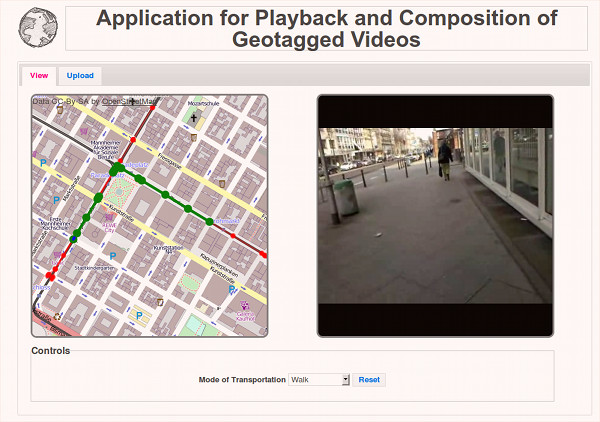
\includegraphics[width=200px]{app_small}
         \caption{Screenshot of original application. Retrieved from \cite{originalsystem}.}
         \label{original-app}
        \end{figure}

We have two main goals we want to achieve with our design. First, visualize points of interest on the map. There should be ways to find relevant information on a point of interest in the application. Secondly, the points of interest should show up on the videos. Such that when a video-clip passes a certain building which is marked as a point of interest a label indicating what point of interest the given building is. 

Regarding finding points of interest this will be done in two steps. First, we have to think about points we consider as relevant and that we want to receive. In the following, we will call these points of interest for POI.  The second step is to get additional information from different data sources referring to the POI. As a result, it is necessary to define an interface which provides additional information relating to the POI to the application. Ideally, the interface is able to request this information from different sources in different data and media types.

In the video, the same POIs as in the map should be visualized when they are in close proximity in front of the camera. The position of a POI should be indicated by if it is shown on the left or the right side of the video. Additionally the distance to the POI can be shown by changing the size of the indicator.

\section{Implementation}

\subsection{Finding points of interest}

The given existing application uses OpenStreetMap (OSM) to visualize available tracks and the current position on the video. It suggests itself to use the available OSM API but according to its documentation, the API is dedicated for editing and not for downloading \cite{osmdata}. Mass requests tend to be resource intensive and since we want to respect this appeal, we use the suggested Overpass API to query for our POI.

The Overpass API supports different Query languages like an XML query format and an own, more concise, query language \cite{overpass-lang}. We recommend to build the queries in the XML format since it is more human readable. The resulting query can be transformed into a concise Overpass query using the given converter. The benefit of using the Overpass query is that it can be performed through a single HTTP request to the interpreter. However, one should pay attention to the number of semicolons at the end of the query as we discovered a little bug due to this work.

Since OSM represents everything with nodes and each node has to be defined by a key-value-pair \cite{osmfeature}, we query for our POI with these key-value-pairs according to a certain radius to our current position. 
The current position is provided by the system with the method call and is needed to build a little bounding box to get the node of the current position from Overpass. Since the box is formed by only two coordinates, it represents the actual point we are looking for. Listing~\ref{lst:xmlquery} and Listing~\ref{lst:overpassquery} show the used query in the current project in XML format as well as in Overpass Query Language.

\begin{lstlisting}[caption={Overpass~query~in~XML~format},label={lst:xmlquery}]
<osm-script output="json">
  <bbox-query s="49.489696" n="49.489696" w="8.467391" e="8.467391"/>
  <query type="node">
    <around radius="1000"/>
    <has-kv k="historic"/>
  </query>
  <print/>
</osm-script>
\end{lstlisting}

\begin{lstlisting}[caption={Overpass~query~in~Overpass~Query~Language},label={lst:overpassquery}]
[out:json];node(49.489827,8.468115,49.489927,8.468215);node(around:1000)["historic"];out;
\end{lstlisting}


The query from Listing~\ref{lst:xmlquery} retrieves nodes with the key ``historic'' and every belonging value (e.g.: monuments, memorials, ruins or shrines) that are around a thousand meters from the Marketplace (G1) in Mannheim. The result will be delivered as a JSON object which will be passed on to other methods in the system that take care of displaying or getting further information. This query represents just a proof of concept but can be easily extended by appending further <query>-tags like in Listing~\ref{lst:xmlquery2}. This query will have the same result as it would be concatenated with an OR-operator. Adding more elements, which can be considered as arguments in this case, into the same <query>-tag will have the same result as an AND-operator.

The Overpass API offers much more possibilities like membership relations between nodes, regular expressions within key-value pairs and unions between queries. Since we consider the explained functions as sufficient to get all interesting geographical points near a given position, we will not go into detail with these sophisticated functions as this is not an introduction to the Overpass API.

\begin{lstlisting}[caption={Enhanced~Overpass~query~in~XML~format},label={lst:xmlquery2}]
<osm-script output="json">
  <bbox-query s="49.489696" n="49.489696" w="8.467391" e="8.467391"/>
  <query type="node">
    <around radius="1000"/>
    <has-kv k="historic"/>
  </query>
  <print/>
  <query type="node">
    <around radius="1000"/>
    <has-kv k="leisure" v="park"/>
  </query>
  <print/>
</osm-script>
\end{lstlisting}


\subsection{Add data to points of interest}

After we download information about the objects nearby, we would like to know more about them and display more information from external sources like Wikipedia or Flickr.

Our aim is to provide an interface capable of doing request for more external APIs. Interface will be implemented in Javascript and will use server support if needed.

Javascript interface is illustrated in Listing~\ref{lst:jsinterface}.

\begin{lstlisting}[caption={Javascript~interface~for~connecting~external~API},label={lst:jsinterface}]
$.info.get = function (api_name, title,	parameters)
\end{lstlisting}

So in order to get Wikipedia content for object with name \textit{NameOfTheObject} you need to call code in Listing~\ref{lst:jsinterfaceexample}.

\begin{lstlisting}[caption={Getting Wikipedia content},label={lst:jsinterfaceexample}]
$.info.get("wikipedia", "NameOfTheObject")
\end{lstlisting}

In order to call Wikipedia API, we wanted to contact its API directly from the Javascript code. The first problem is that we are requesting data from different domain, so in order to avoid cross-domain problems we used \textit{JSONP} to get the data.

After solving this issue, data we are getting are still in the Wikimedia format, which needs to be parsed by the client.

At the end, we decided to have a support for the Wikipedia API on the server side, because we can use Python packages like \textit{wikitools} to work with Wikipedia API in a more elegant way.

Data we gather from the APIs will be part of the tooltips visible in the video and on the map. For now we support Wikipedia API, but it's possible to easily add other APIs.

Each API will have to be treated individually, some of them will require server support also because of the API keys, some of them will require caching of the data because of the API limitations. What we require from the future implementations is to follow the defined interface, so that developers can always rely on that kind of abstraction.

\subsection{Displaying POIs on the map}

This part drafts how the system displays points of interest on the map. It was not sufficient enough to implement a method that adds markers to the map as changes to the core of the system were needed. First of all, it was necessary to add another layer for the markers that should be drawn by the OpenLayers API. Furthermore the depth of this layer had to be set, so a popup would appear after a click on the marker. If the Layer is not correctly initialized, the application will not recognize any motion on this layer.

As these changes were performed, the marker drawing function \textit{setMarker} could be implemented. This function is called from the success function of the performed AJAX call in \textit{onVideoProgress} after the POIs were received from the Overpass API. The points the system is interested in are stored in a JSON object. This object will be iterated to get the longitude, the latitude and the name. These are the parameters that are required to create and set a marker with an associated popup. Afterwards the method adds an event to the popup in case the mouse moves over the marker.

All in all, after the core of the system has been modified, markers can be added to the map very easily. However, the documentation of the OpenLayers API is very poor. This fact turned this easy looking part of displaying markers on a map into a real challenge.


\subsection{Displaying POIs in the video}

Once we have all the data available locally in the web browser, it's time to visualize them on the video. 

In the existing system, the HTML5 video tag is used for displaying the video content. The idea is to add HTML overlay over this video and display custom content there. This task thus consists of three different sub-tasks.

	\begin{list}{\textbullet}{}
		\item Overlaying HTML5 video tag
		\item Filtering the places which are visible in the video
		\item Displaying data in the video overlay
	\end{list}

\subsubsection{Overlaying HTML5 video tag}

For this task we will just construct \textit{div} tag with id \textit{video-wrapper} with \textit{relative} positioning. This wrapper will contain two elements - video tag and another \textit{div} tag with id \textit{video-overlay}.

Since video wrapper will have relative positioning, all we need is to make sure that video overlay has higher \textit{z-index} and we can add objects here which will be visible above the video tag.

The only complication which can happen with this solution is bad behavior during fullscreen mode.

If we want to make video fullscreen, we would loose the objects, because they are just placed in another layer. Solution is to use HTML5 \textit{requestFullscreen} function. If we want to make video fullscreen, we will need to call HTML5 \textit{requestFullscreen} function on the video wrapper element, since it contains both the video and the overlay. It's important to mention that \textit{requestFullscreen} function is only triggerable via user input (i.e. clicking the button), because of the security.

\subsubsection{Filtering visible places}

We have already fetched all the interesting information about objects nearby. If we want to now display them above the video, we need to know which objects are actually nearby or visible.

If we know which places are nearby, we can display some tips in the video. For the objects that can be visible on the video, we will try to estimate their location in the video.

In the objects fetched from the external API, we are provided with the coordinates of each object. Since we need to recalculate the current view every time we have moved in the video, we will create a function \textit{showPlacesOnTheVideo} which will be called from within already provided \textit{onVideoProgress} function.

	This function is great place to do these kind of calculations, because it is called every time the video proceeds a new point on the map. Updating the view on the video in this interval is thus sufficient. If more precise calculations will be needed in the future, it is possible just to call \textit{showPlacesOnTheVideo} function more times using the timer.
	
	In the \textit{onVideoProgress} function, we are already provided with the current point and the next point we are about to reach. Now we know where are we located, our direction and places nearby.

\paragraph{Getting the places nearby}

In order to get all the nearby places, we need to iterate through them and check if 


\begin{displaymath}
abs(current.lon - place.lon) \leq r
\end{displaymath}
and
\begin{displaymath}
abs(current.lat - place.lat) \leq r
\end{displaymath}

 where \textit{current} is object containing our coordinates, \textit{place} is the object containing the coordinates of the place we are interested in and \textit{r} is a constant defining the acceptable difference for the coordinates, which is set to \textit{0.0009} by default.

\paragraph{Getting the places in front of us}

As seen on Figure~\ref{filtering}, we will know the coordinates of the current point and the point we are about to reach. What we want to count are points A, B, C and D. If we can calculate the positions of these points, we will be able to say that the object is in front of us, if it's located withing this rectangle.

We will be also able to say whether an object is located on the right side of the video or the left side of the video, depending on which of the areas of the rectangle contains the object. We will be also able to return the distance from the object, which can be useful while rendering the object on the video.

After recalculating, we will be able to say whether the object is located on the right or left side of the street and say how far away it is. Which should be sufficient for estimating its position within video overlay.

        \begin{figure}[htb]
         \centering
         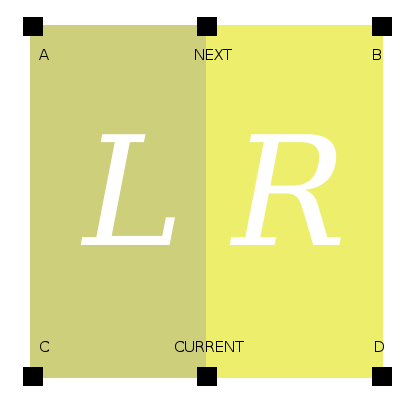
\includegraphics[width=200px]{filtering}
         \caption{Calculating the places in front of us}
         \label{filtering}
        \end{figure}
        
In order to do this we need to first calculate vector of our direction vector.

\begin{displaymath}
CURRENT = [lat, lon]
\end{displaymath}
\begin{displaymath}
NEXT = [lat, lon]
\end{displaymath}
\begin{displaymath}
\vec{direction} = (CURRENT, NEXT)
\end{displaymath}

When we have the direction vector, we can calculate the normal vectors.

\begin{displaymath}
\vec{n1} = (-direction[1], direction[0])
\end{displaymath}
\begin{displaymath}
\vec{n2} = (direction[1], -direction[0])
\end{displaymath}

If we add normal vectors to the points \textit{NEXT} and \textit{CURRENT} we can calculate the coordinates of \textit{A}, \textit{B}, \textit{C} and \textit{D}

\begin{displaymath}
A[0] = NEXT[0] + n1[0]*c
\end{displaymath}
\begin{displaymath}
A[1] = NEXT[1] + n1[1]*c
\end{displaymath}

where \textit{c} is the constant specifying the width of our view.

Once we have calculated all of the coordinates, we can say whether object we are trying to locate is within the range and if so we can analyze whether it is on the right side or left side of the view.

Since we know the \textit{CURRENT} coordinates and coordinates of the video we can also return the distance of the objects from our current location.

In case we want to specify wider or longer view range. We can move the NEXT point by adding the direction vector for longer range or we can specify higher \textit{c} constant for wider range.

Constant \textit{c} is initially set to 1, which means that distance between points \textit{CURRENT} and \textit{NEXT} is the same as distance between points \textit{NEXT} and \textit{B}.

\subsubsection{Displaying data in the video overlay}

After we are done with calculations and we can say about each object whether it is located in front of us or not, we can start visualizing these elements on the video overlay.

Properties we have determined for each object are it's distance, information whether it is on the right or left side of the street and other properties like name and type of the object we fetched from the external APIs.

It is important to realize that video may have different dimensions so all of the positioning needs to be done in the relative way.

We will set CSS \textit{float} attribute to \textit{left} or \textit{right} for all the objects depending on their positions and will set up their size and position depending on the distance of the object.

Our assumption is that this system will be used mostly in streets so specifying that something is on the right side or the left side should be sufficient.

\section{Evaluation}

\subsection{Points of interest and language}

        \begin{figure}[htb]
         \centering
         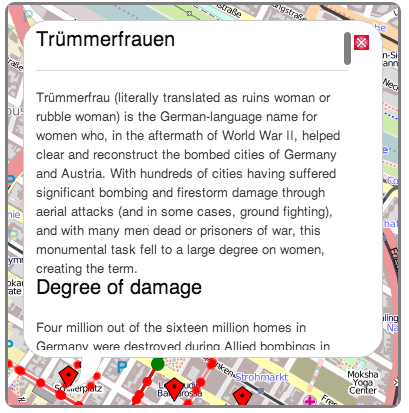
\includegraphics[width=200px]{popup_with_content}
         \caption{Point of interest popup with english Wikipedia content.}
         \label{popup_with_content}
        \end{figure}


We tested our system with videos from Mannheim in Germany. When querying for historical points of interest from Overpass\cite{overpass} our result set consisted of only german names for places. When displaying information in popups on the map we combine the name from points of interest with text retrieved from Wikipedia API\cite{wikiapi}. Wikipedia was queried by using the name of the point of interest. Figure~\ref{popup_with_content} show a popup where english Wikipedia content was found. As the names of the points of interest where in german and we query the english Wikipedia we rarely got any hits. Figure~\ref{popup_with_content} was actually one of the very few points of interest with english wikipedia content. Figure~\ref{popup_wo_content} displays a popup where there was not found any Wikipedia information.

        \begin{figure}[htb]
         \centering
         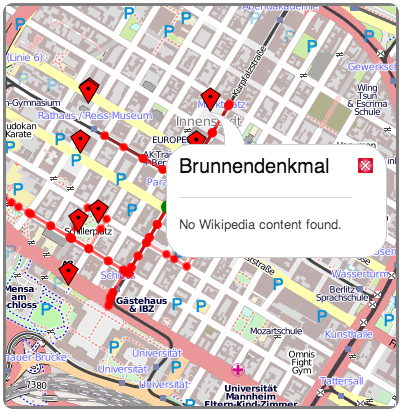
\includegraphics[width=200px]{popup_wo_content}
         \caption{Point of interest popup where no english Wikipedia content was found.}
         \label{popup_wo_content}
        \end{figure}


\section{Conclusion}
The conclusion goes here.





% if have a single appendix:
%\appendix[Proof of the Zonklar Equations]
% or
%\appendix  % for no appendix heading
% do not use \section anymore after \appendix, only \section*
% is possibly needed

% use appendices with more than one appendix
% then use \section to start each appendix
% you must declare a \section before using any
% \subsection or using \label (\appendices by itself
% starts a section numbered zero.)
%


\appendices
\section{Proof of the First Zonklar Equation}
Appendix one text goes here.

% you can choose not to have a title for an appendix
% if you want by leaving the argument blank
\section{}
Appendix two text goes here.


% use section* for acknowledgement
\section*{Acknowledgment}


The authors would like to thank...


% Can use something like this to put references on a page
% by themselves when using endfloat and the captionsoff option.
\ifCLASSOPTIONcaptionsoff
  \newpage
\fi



% trigger a \newpage just before the given reference
% number - used to balance the columns on the last page
% adjust value as needed - may need to be readjusted if
% the document is modified later
%\IEEEtriggeratref{8}
% The "triggered" command can be changed if desired:
%\IEEEtriggercmd{\enlargethispage{-5in}}

% references section

% can use a bibliography generated by BibTeX as a .bbl file
% BibTeX documentation can be easily obtained at:
% http://www.ctan.org/tex-archive/biblio/bibtex/contrib/doc/
% The IEEEtran BibTeX style support page is at:
% http://www.michaelshell.org/tex/ieeetran/bibtex/
%\bibliographystyle{IEEEtran}
% argument is your BibTeX string definitions and bibliography database(s)
%\bibliography{IEEEabrv,../bib/paper}
%
% <OR> manually copy in the resultant .bbl file
% set second argument of \begin to the number of references
% (used to reserve space for the reference number labels box)


\begin{thebibliography}{1}

\bibitem{osmdata}
(2013, Apr.) OpenStreetMap wiki about how to download data. [Online]. Available: \url{http://wiki.openstreetmap.org/wiki/Getting_Data}

\bibitem{osmfeature}
(2013, Apr.) OpenStreetMap wiki about the tagging system. [Online]. Available: \url{http://wiki.openstreetmap.org/wiki/Map_Features}

\bibitem{overpass-lang}
(2013, Apr.) Overpass API language guide. [Online]. Available: \url{http://wiki.openstreetmap.org/wiki/Overpass_API/Language_Guide}

\bibitem{flickr}
(2013, Apr.) Flickr. \url{http://www.flickr.com/}

\bibitem{youtube}
(2013, Apr.) YouTube. \url{http://www.youtube.com/}

\bibitem{foursquare}
(2013, Apr.) Foursqaure. \url{http://www.foursquare.com/}

\bibitem{overpass}
(2013, Apr.) OpenStreetMap Overpass API. \url{http://wiki.openstreetmap.org/wiki/Overpass_API}

\bibitem{placing-meta-on-map}
Spyrou, E., and Mylonas, P. (2011, December). Placing User-Generated Photo Metadata on a Map. In Semantic Media Adaptation and Personalization (SMAP), 2011 Sixth International Workshop on (pp. 79-84). IEEE.

\bibitem{geotagging-survey}
Luo, J., Joshi, D., Yu, J., and Gallagher, A. (2011). Geotagging in multimedia and computer vision?a survey. Multimedia Tools and Applications, 51(1), 187-211.

\bibitem{geonames}
(2013, Apr.) Geonames. \url{http://www.geonames.org/}

\bibitem{next-vacation}
Kisilevich, S., Mansmann, F., Bak, P., Keim, D., and Tchaikin, A. (2010, February). Where would you go on your next vacation? A framework for visual exploration of attractive places. In Advanced Geographic Information Systems, Applications, and Services (GEOPROCESSING), 2010 Second International Conference on (pp. 21-26). IEEE.

\bibitem{collective-photography}
Chippendale, P., Zanin, M., and Andreatta, C. (2009, November). Collective photography. In Visual Media Production, 2009. CVMP'09. Conference for (pp. 188-194). IEEE.

\bibitem{google-earth}
(2013, Apr.) Google Earth. \url{http://www.google.com/earth/index.html}

\bibitem{twitter}
(2013, Apr.) Twitter. \url{http://www.twitter.com}

\bibitem{facebook}
(2013, Apr.) Facebook. \url{http://www.facebook.com}

\bibitem{originalsystem}
http://ls.wim.uni-mannheim.de/de/pi4/research/projects/geotagged-videos

\bibitem{wikiapi}



\end{thebibliography}



% biography section
% 
% If you have an EPS/PDF photo (graphicx package needed) extra braces are
% needed around the contents of the optional argument to biography to prevent
% the LaTeX parser from getting confused when it sees the complicated
% \includegraphics command within an optional argument. (You could create
% your own custom macro containing the \includegraphics command to make things
% simpler here.)
%\begin{biography}[{\includegraphics[width=1in,height=1.25in,clip,keepaspectratio]{mshell}}]{Michael Shell}
% or if you just want to reserve a space for a photo:

%\begin{IEEEbiography}{Michael Shell}
%Biography text here.
%\end{IEEEbiography}

% if you will not have a photo at all:
%\begin{IEEEbiographynophoto}{John Doe}
%Biography text here.
%\end{IEEEbiographynophoto}

% insert where needed to balance the two columns on the last page with
% biographies
%\newpage

%\begin{IEEEbiographynophoto}{Jane Doe}
%Biography text here.
%\end{IEEEbiographynophoto}

% You can push biographies down or up by placing
% a \vfill before or after them. The appropriate
% use of \vfill depends on what kind of text is
% on the last page and whether or not the columns
% are being equalized.

%\vfill

% Can be used to pull up biographies so that the bottom of the last one
% is flush with the other column.
%\enlargethispage{-5in}



% that's all folks
\end{document}


